\documentclass{article}

% Required packages (merged from hw5_template.tex and hw6_questions.tex)
\usepackage{amssymb}
\usepackage{amsmath}
\usepackage{graphicx}
\usepackage{geometry}
\usepackage{tikz}
\usepackage{array}
\usepackage{booktabs}
\usepackage{enumitem}
\usepackage{listings}
\usepackage{xcolor}
\usepackage{fancyhdr}
\usepackage{float}
\usepackage{subcaption}
\usepackage{comment}
\usepackage{algorithm}
\usepackage{algpseudocode}
\usepackage{caption}
\usepackage{siunitx}
\usepackage{hyperref}
\usetikzlibrary{arrows.meta, positioning} % Required for hw6 diagrams

% Set page geometry
\geometry{a4paper, margin=1in}

% Configure listings for Python
\lstset{
  language=Python,
  basicstyle=\ttfamily\footnotesize,
  numbers=left,
  numberstyle=\tiny\color{gray},
  frame=single,
  breaklines=true,
  breakatwhitespace=true,
  captionpos=b,
  tabsize=4,
  showspaces=false,
  showstringspaces=false,
  showtabs=false,
  commentstyle=\color{gray}\textit,
  keywordstyle=\color{blue}\bfseries,
  stringstyle=\color{red}
}

\begin{document}

\pagestyle{fancy}
\chead{DSC 257: Unsupervised Learning (Fall 2025)}
\lhead{Homework 6}
\rhead{Randall Rogers}

%------------------
% Solution for 1(a)
%------------------
\subsection*{Solution 1}
\noindent\rule{\textwidth}{0.4pt}\\
\subsubsection*{Solution 1 (a)}
\subsubsection*{Python Code}
\begin{lstlisting}[language=Python]
import numpy as np
import matplotlib.pyplot as plt

# set random seed 
np.random.seed(42)

# define pi, mu, sigma 
pi = np.array([0.1, 0.2, 0.5, 0.2])
mu = [np.array([7, 6]), np.array([0, 0]), np.array([-1, 4]), np.array([5, -2])]
sigma = [np.array([[1, 0], [0, 25]]), np.array([[1, 0], [0, 1]]),
    np.array([[9, 1], [1, 1]]), np.array([[16, -6], [-6, 4]])]

# generate 400 random points from the mixture model
N = 400
z_labels = np.random.choice(len(pi), size=N, p=pi)

# make containers for X data ,true labels data
X_data = []
true_labels = []

# sample from the specific Gaussian for each component
for i in range(4):
    # Count how many points belong to component i
    n_i = np.sum(z_labels == i)
    if n_i > 0:
        # Sample n_i points from N(mu_i, Sigma_i)
        pts = np.random.multivariate_normal(mu[i], sigma[i], n_i)
        X_data.append(pts)
        true_labels.append(np.full(n_i, i))

# massage data for plots
X = np.vstack(X_data)
y = np.concatenate(true_labels)

# plot points, using colors to distinguish each of the components
plt.figure(figsize=(8, 6))
colors = ['red', 'green', 'blue', 'orange']
labels = ['$\pi_1 N(\mu_1, \Sigma_1)$', '$\pi_2 N(\mu_2, \Sigma_2)$', 
    '$\pi_3 N(\mu_3, \Sigma_3)$', '$\pi_4 N(\mu_4, \Sigma_4)$']

for i in range(4):
    plt.scatter(X[y == i, 0], X[y == i, 1], 
    c=colors[i], label=labels[i], alpha=0.6, s=20)

plt.title('Q1(a): Generated Data from 4-Component GMM')
plt.xlabel('X1')
plt.ylabel('X2')
plt.xlim(-15,18)
plt.ylim(-7,18)
plt.legend()
plt.grid(True, alpha=0.3)
plt.savefig('q1a.png') # Save for LaTeX inclusion
\end{lstlisting}

\newpage

\subsection*{Solution 1}
\noindent\rule{\textwidth}{0.4pt}\\
\subsubsection*{Solution 1 (a)}
\subsubsection*{Plot}
% Ensure the file q1a.png exists in your directory after running the code
\begin{figure}[h]
\centering
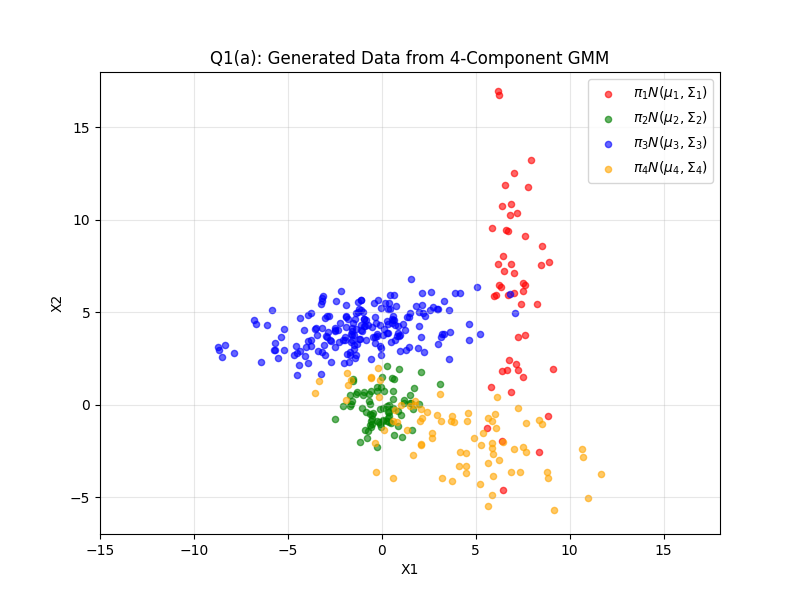
\includegraphics[width=0.9\textwidth]{q1a.png} 
% Note: Uncomment the line above once you have generated the image
\caption{Visualization of the 400 random points generated from the mixture model.}
\label{fig:1a}
\end{figure}

\noindent\rule{\textwidth}{0.4pt}\\

\newpage

%------------------
% Solution for 1(b)
%------------------
\subsection*{Solution 1}
\noindent\rule{\textwidth}{0.4pt}\\
\subsubsection*{Solution 1 (b)}
\subsubsection*{Python Code}
\begin{lstlisting}[language=Python]
import numpy as np
import matplotlib.pyplot as plt
from matplotlib.patches import Ellipse

# set random seed 
np.random.seed(42)

# define pi, mu, sigma 
pi = np.array([0.1, 0.2, 0.5, 0.2])
mu = [np.array([7, 6]), np.array([0, 0]), np.array([-1, 4]), np.array([5, -2])]
sigma = [np.array([[1, 0], [0, 25]]), np.array([[1, 0], [0, 1]]),
    np.array([[9, 1], [1, 1]]), np.array([[16, -6], [-6, 4]])]

# generate 400 random points from the mixture model
N = 400
z_labels = np.random.choice(len(pi), size=N, p=pi)

# make containers for X data ,true labels data
X_data = []
true_labels = []

# sample from the specific Gaussian for each component
for i in range(4):
    # Count how many points belong to component i
    n_i = np.sum(z_labels == i)
    if n_i > 0:
        # Sample n_i points from N(mu_i, Sigma_i)
        pts = np.random.multivariate_normal(mu[i], sigma[i], n_i)
        X_data.append(pts)
        true_labels.append(np.full(n_i, i))

# massage data for plots
X = np.vstack(X_data)
y = np.concatenate(true_labels)

def plot_ellipse(mu, sigma, ax, color):
    # calc eigen values/vectors
    vals, vecs = np.linalg.eigh(sigma)
    
    # Sort eigenvalues/vectors large -> small 
    order = vals.argsort()[::-1]
    vals = vals[order]
    vecs = vecs[:, order]
    
    # calc angle
    theta = np.degrees(np.arctan2(*vecs[:,0][::-1]))
    
    # calc width and height based on eigenvalues
    width, height = 2.0 * np.sqrt(3.0 * vals)
    
    # create ellipse
    ell = Ellipse(xy=mu, width=width, height=height, angle=theta, 
                  edgecolor=color, facecolor='none', lw=2, label='_nolegend_')
    ax.add_artist(ell)

# make plot
fig, ax = plt.subplots(figsize=(8, 6))
colors = ['red', 'green', 'blue', 'orange']
labels = ['$\pi_1 N(\mu_1, \Sigma_1)$', '$\pi_2 N(\mu_2, \Sigma_2)$', 
    '$\pi_3 N(\mu_3, \Sigma_3)$', '$\pi_4 N(\mu_4, \Sigma_4)$']

for i in range(4):
    plt.scatter(X[y == i, 0], X[y == i, 1], c=colors[i], 
        label=labels[i], alpha=0.6, s=20)
    plot_ellipse(mu[i], sigma[i], ax, color=colors[i])
    # mark center of ellipse
    ax.scatter(mu[i][0], mu[i][1], c='black', marker='x', s=50)

plt.title('Q1(b): Data Points with Covariance Ellipses')
plt.xlabel('X1')
plt.ylabel('X2')
plt.legend()
plt.grid(True, alpha=0.3)
plt.axis('equal') 
plt.savefig('q1b.png')
\end{lstlisting}

\subsubsection*{Plot}
% Ensure the file q1b.png exists in your directory after running the code
\begin{figure}[h!]
\centering
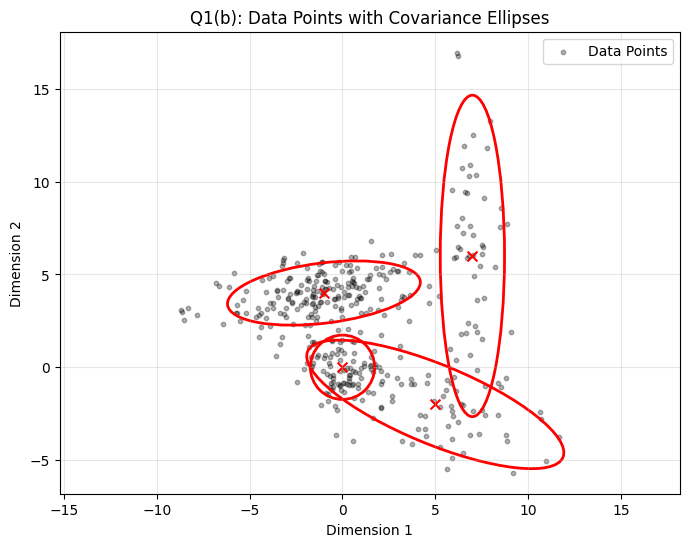
\includegraphics[width=0.9\textwidth]{q1b.png}
% Note: Uncomment the line above once you have generated the image
\caption{Visualization of the 400 random points (black) overlaid with red ellipses representing the 99\% confidence intervals of the four Gaussian components.}
\label{fig:1b}
\end{figure}

\noindent\rule{\textwidth}{0.4pt}\\

\newpage

%------------------
% Solution for 1(c)
%------------------
\subsection*{Solution 1}
\noindent\rule{\textwidth}{0.4pt}\\
\subsubsection*{Solution 1 (c)}
\subsubsection*{Plot}
\begin{figure}[h!]
\centering
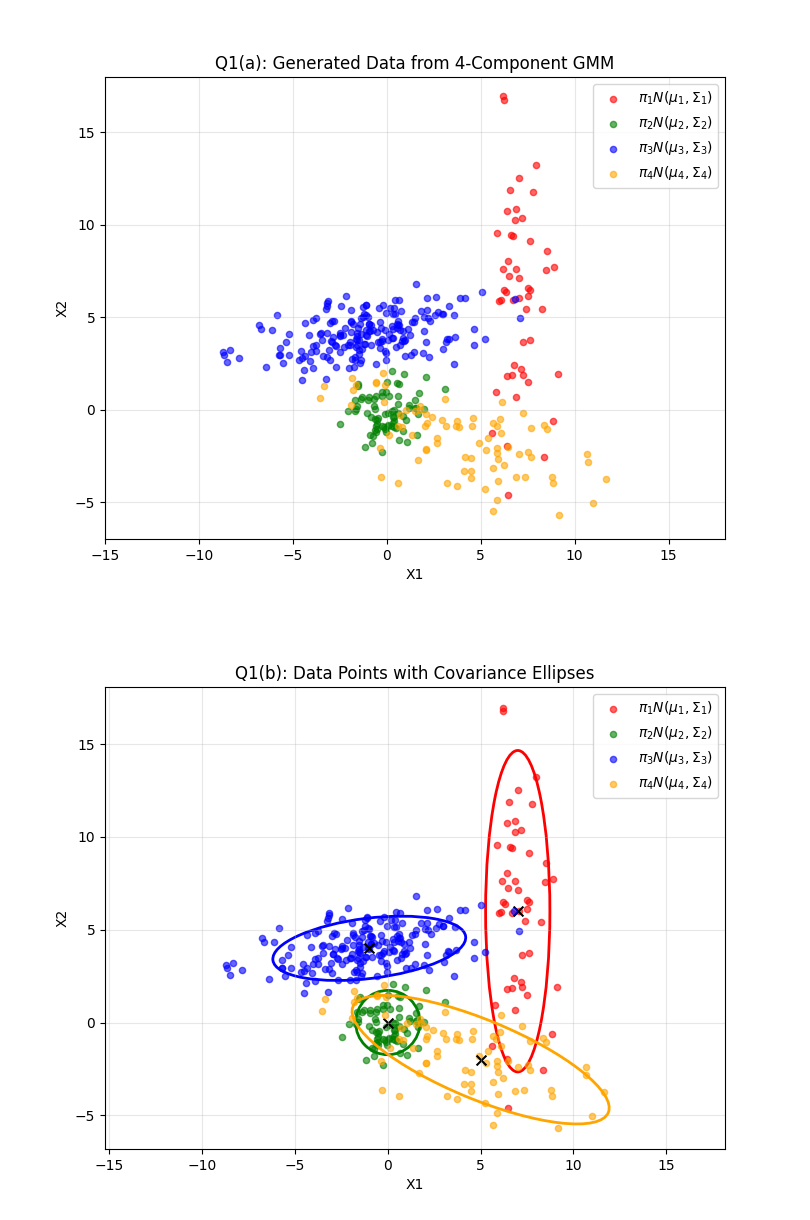
\includegraphics[width=0.7\textwidth]{q1c.png} 
\caption{Comparison of plots from \textit{part (a)} and \textit{part (b)}. The \textit{2nd Cluster} (Green, $\mu_2=[0,0]$) is the small cluster that is partially contained by the \textit{4th Cluster} (Orange, $\mu_4=[5,-2]$)}
\label{fig:q1c}
\end{figure}

\noindent\rule{\textwidth}{0.4pt}\\

\newpage

%------------------
% Solution for 1(d)
%------------------
\subsection*{Solution 1}
\noindent\rule{\textwidth}{0.4pt}\\
\subsubsection*{Solution 1 (d)}
\subsubsection*{Python Code}

\begin{lstlisting}[language=Python]
from sklearn.mixture import GaussianMixture

# initialize and fit the GMM
gmm = GaussianMixture(n_components=4, covariance_type='full', random_state=42)
gmm.fit(X) 

fig2, ax2 = plt.subplots(figsize=(10, 8))

# plot orginal data
ax2.scatter(X[:, 0], X[:, 1], c='gray', s=15, alpha=0.2, label='Observed Data')

# plot true
for i in range(4):
    plot_ellipse(mu[i], sigma[i], ax2, color=colors[i], linestyle='solid', linewidth=1.5)
    # add filler for legend
    ax2.scatter([], [], c=colors[i], label=f'True Comp {i+1}')

# plot model
for i in range(4):
    learned_mean = gmm.means_[i]
    learned_cov = gmm.covariances_[i]
    
    # plot learned ellipse
    plot_ellipse(learned_mean, learned_cov, ax2, color='black', linestyle='--', linewidth=2.5)
    
    # mark learned centers
    label = 'Learned Parameters' if i == 0 else ""
    ax2.scatter(learned_mean[0], learned_mean[1], c='black', 
                marker='+', s=120, lw=2, label=label)

ax2.set_title('Q1(d): Comparison of Learned (Black/Dashed) vs True (Color/Solid)', fontsize=14)
ax2.set_xlabel('X1')
ax2.set_ylabel('X2')
ax2.axis('equal')
ax2.grid(True, alpha=0.3)
ax2.legend(loc='upper right')
plt.savefig('q1d.png')
\end{lstlisting}

\newpage

\subsection*{Solution 1}
\noindent\rule{\textwidth}{0.4pt}\\
\subsubsection*{Solution 1 (d)}

\subsubsection*{Plot}
% Ensure q1d.png is generated
\begin{figure}[h!]
\centering
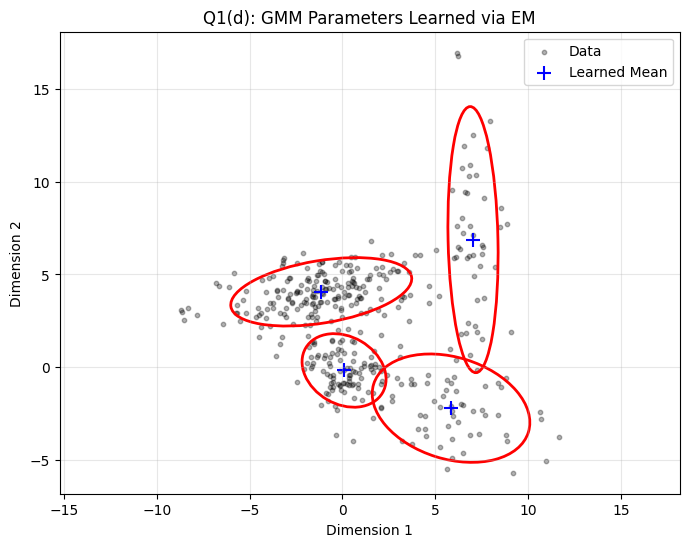
\includegraphics[width=0.7\textwidth]{q1d.png}
\caption{Visualization of the ellipses learned by the EM algorithm (blue crosses denote learned means) overlaid on the original data.}
\label{fig:q1d}
\end{figure}

\subsubsection*{\normalfont}{$\therefore$ The Gaussians learned by the EM algorithm are close to the true generative parameters, with only minor deviations due to noise and sample size.}

\noindent\rule{\textwidth}{0.4pt}\\

\newpage

%------------------
% Solution for 1(e)
%------------------
\subsection*{Solution 1}
\noindent\rule{\textwidth}{0.4pt}\\
\subsubsection*{Solution 1 (e)}
\subsubsection*{Python Code}

\begin{lstlisting}[language=Python]
from sklearn.mixture import GaussianMixture

# initialize and fit the GMM
gmm = GaussianMixture(n_components=4, covariance_type='full', random_state=42)
gmm.fit(X)

# make predictions
y_pred = gmm.predict(X)

# plot predictions
plt.figure(figsize=(8, 6))

# define colors for predicted data
colors_pred = ['purple', 'cyan', 'lime', 'magenta'] 
for k in range(4):
    # select points predicted to belong to cluster k
    mask = (y_pred == k)
    plt.scatter(X[mask, 0], X[mask, 1], s=20, label=f'Cluster {k}', alpha=0.6)

plt.title('Q1(e): Data Colored by GMM Hard Clustering')
plt.xlabel('X1')
plt.ylabel('X2')
plt.legend()
plt.grid(True, alpha=0.3)
plt.savefig('q1e.png')
plt.show()
\end{lstlisting}

\newpage

\subsection*{Solution 1}
\noindent\rule{\textwidth}{0.4pt}\\
\subsubsection*{Solution 1 (e)}
\subsubsection*{Plot}
% Ensure q1e.png is generated
\begin{figure}[h!]
\centering
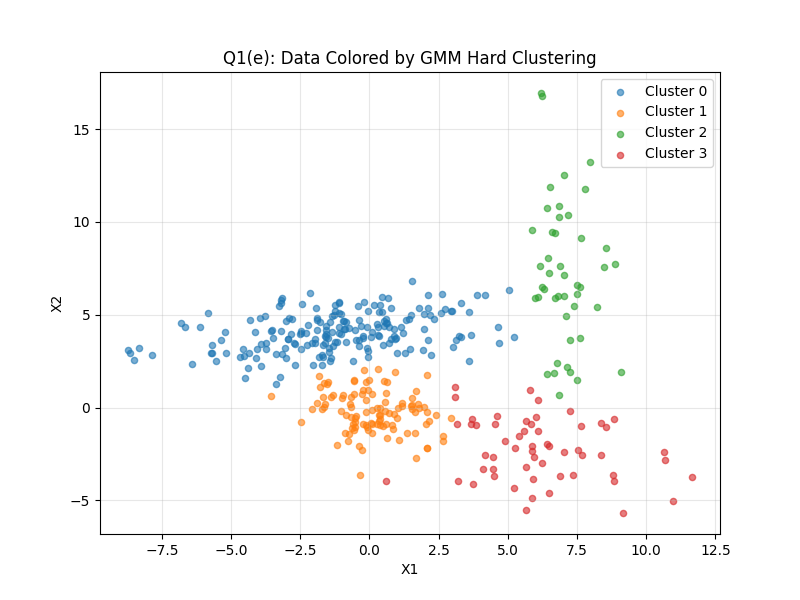
\includegraphics[width=0.7\textwidth]{q1e.png}
\caption{Visualization of the data points colored by their assigned cluster (Hard Assignment).}
\label{fig:q1e}
\end{figure}

\subsubsection*{Plot Comments}
\begin{flushleft}
    The clustering is not perfect, but it captures the general structure of the data well.
\end{flushleft}


\begin{flushleft}
    The discrepancies are understandable since this happens where there is overlap.
\end{flushleft}

\noindent\rule{\textwidth}{0.4pt}\\

\newpage

%------------------
% Solution for 1(f)
%------------------
\subsection*{Solution 1}
\noindent\rule{\textwidth}{0.4pt}\\
\subsubsection*{Solution 1 (f)}
\subsubsection*{Python Code}

\begin{lstlisting}[language=Python]
import warnings
from sklearn.mixture import GaussianMixture

# set iteration snapshots 
iterations = [1, 5, 10, 50] 

plt.figure(figsize=(15, 10))

for idx, n_iter in enumerate(iterations):
    # initialize GMM 
    gmm = GaussianMixture(n_components=4, 
                          covariance_type='full', 
                          max_iter=n_iter, 
                          random_state=42,
                          init_params='random')
    
    # suppress warnings
    with warnings.catch_warnings():
        warnings.simplefilter("ignore")
        gmm.fit(X)
    
    # plot subplot
    ax = plt.subplot(2, 2, idx+1)
    ax.scatter(X[:, 0], X[:, 1], c='k', s=5, alpha=0.2)
    
    # plot learned ellipses
    for i in range(4):
        plot_ellipse(gmm.means_[i], gmm.covariances_[i], ax)
        ax.scatter(gmm.means_[i][0], gmm.means_[i][1], c='blue', marker='+')
        
    ax.set_title(f'Iteration {n_iter}')
    ax.axis('equal')

plt.tight_layout()
plt.savefig('q1f_evolution.png')
plt.show()
\end{lstlisting}

\newpage

\subsection*{Solution 1}
\noindent\rule{\textwidth}{0.4pt}\\
\subsubsection*{Solution 1 (f)}
\subsubsection*{Plot}
% Ideally, display the 4 snapshots. 
% If you saved them as one combined image:
\begin{figure}[h!]
\centering
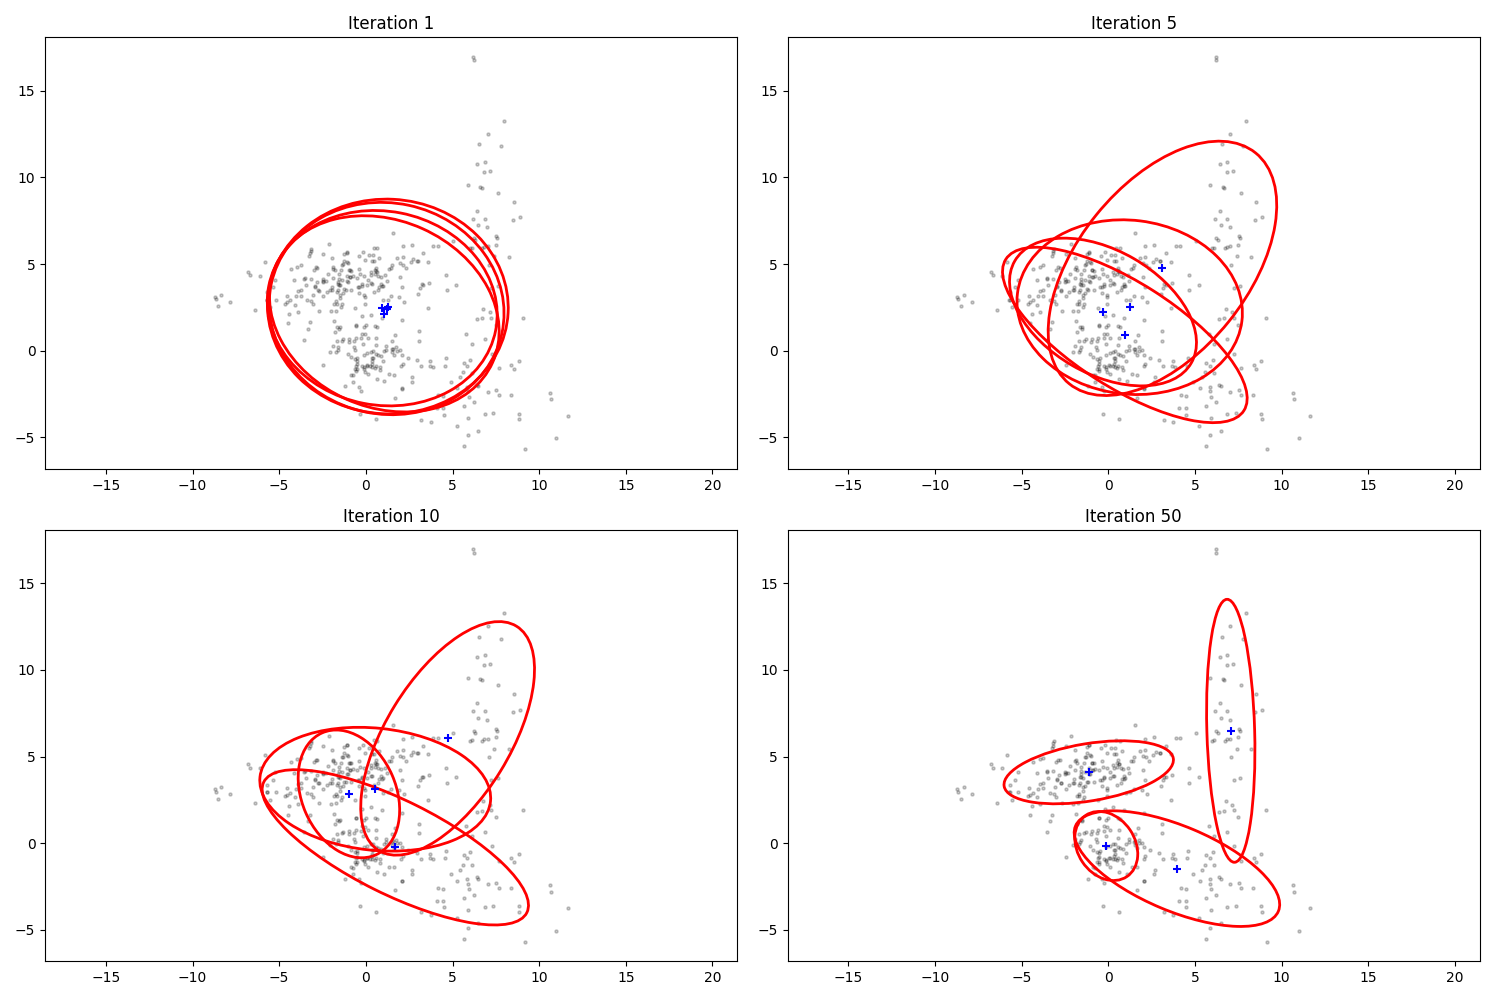
\includegraphics[width=1.0\textwidth]{q1f_evolution.png}
\caption{Evolution of the EM algorithm at iterations 1, 5, 10, and 50.}
\label{fig:q1f}
\end{figure}

\noindent\rule{\textwidth}{0.4pt}\\

\newpage


%------------------
% Solution for 2(a)
%------------------
\subsection*{Solution 2}
\noindent\rule{\textwidth}{0.4pt}\\
\subsubsection*{Question 2 (a)}
\begin{flushleft}
\textit{Kernel density estimation:} Suppose we have samples $x_1, x_2, \ldots, x_n \in \mathbb{R}^d$ from an unknown distribution $f$, and we want to come up with a model of $f$. One simple way to do this is using the kernel density estimator $\widehat{f}$, which approximates $f$ using a mixture of $n$ Gaussians, each with weight $1/n$, and each centered at one of the data points:
\end{flushleft}
$$\widehat{f}: \frac{1}{n} N(x_1, \sigma^2 I_d) + \frac{1}{n} N(x_2, \sigma^2 I_d) + \cdots + \frac{1}{n} N(x_n, \sigma^2 I_d)$$
\begin{flushleft}
    Here $\sigma$ must be selected carefully. It is usually called the bandwidth parameter.
\end{flushleft}
\begin{figure}[h!]
\centering
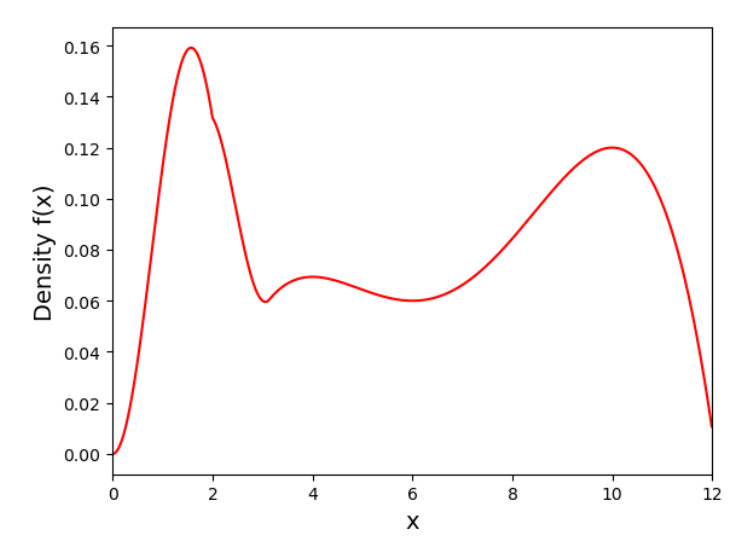
\includegraphics[width=0.7\textwidth]{q2.png}
\caption{The file \texttt{samples.txt} contains 1,000 samples drawn from $f$ (using rejection sampling).}
\label{fig:q2}
\end{figure}
\begin{itemize}
    \item Plot a histogram of the 1,000 samples using 20 bins.It should (very roughly) resemble the distribution f shown above.
\end{itemize}
\subsubsection*{Solution 2 (a)}
\subsubsection*{Python Code}

\begin{lstlisting}[language=Python]
import numpy as np
import matplotlib.pyplot as plt

# Load the data from the provided text file
# Ensure 'samples.txt' is in the same directory as this script
try:
    data = np.loadtxt('samples.txt')
except FileNotFoundError:
    print("Error: samples.txt not found. Please ensure the file is in the working directory.")
    # Fallback for demonstration if file is missing (generating similar synthetic data)
    # data = np.concatenate([np.random.normal(1.5, 0.5, 300), np.random.normal(10, 1, 400), np.random.normal(4, 1, 300)])
    data = np.array([])

if len(data) > 0:
    plt.figure(figsize=(8, 6))
    
    # Plot histogram with 20 bins
    # density=True normalizes the counts to form a probability density
    # This makes the y-axis comparable to the "Density f(x)" plot in the question
    plt.hist(data, bins=20, density=True, color='skyblue', edgecolor='black', alpha=0.7)
    
    plt.title('Q2(a): Histogram of 1,000 Samples (20 Bins)')
    plt.xlabel('Value (x)')
    plt.ylabel('Density')
    plt.grid(True, alpha=0.3)
    plt.xlim(0, 12)  # Matching the range of the reference image q2.png
    
    plt.savefig('q2a.png')
    plt.show()
\end{lstlisting}

\subsubsection*{Plot}
% Ensure q2a.png is generated
\begin{figure}[h!]
\centering
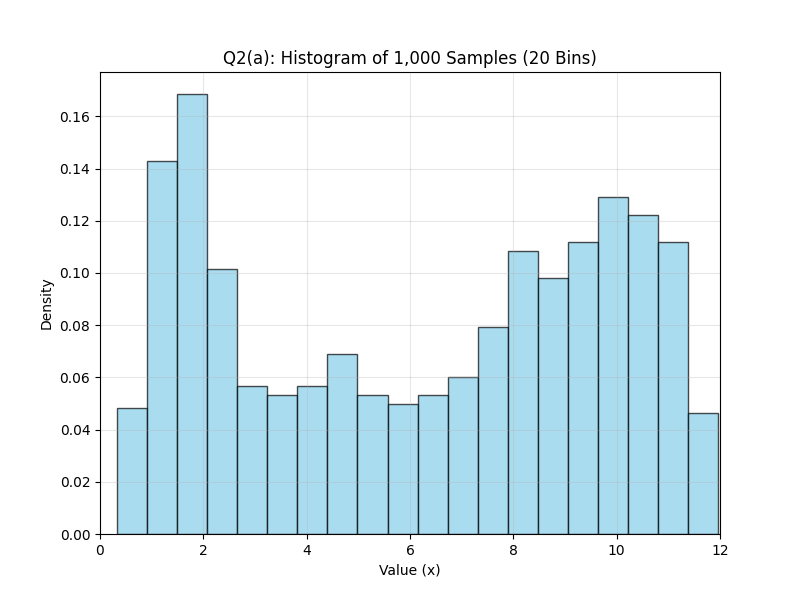
\includegraphics[width=0.7\textwidth]{q2a.png}
\caption{Histogram of the 1,000 samples using 20 bins. Note the bimodal structure roughly resembling the distribution $f$.}
\label{fig:q2a}
\end{figure}


\subsubsection*{\normalfont}{$\therefore$ }
The histogram approximates the underlying distribution $f$. We observe a high density peak in the region $x \in [1, 2]$ and a broader, secondary mode around $x \in [9, 11]$. The region around $x=6$ has lower density. This structure roughly mirrors the "True Density" shown in Figure \ref{fig:q2}.

\subsubsection*{Graduate Level Explanation}
A histogram is the simplest form of **Non-Parametric Density Estimation**. It partitions the sample space into disjoint hypercubes (bins) of volume $V$ (here, interval width $h$) and estimates the density as $\hat{p}(x) = \frac{k}{NV}$, where $k$ is the number of samples in the bin containing $x$.
While intuitive, histograms suffer from two main drawbacks:
\begin{enumerate}
    \item **Discontinuity:** The resulting density function is a step function, which is not smooth (not differentiable).
    \item **Dependency on Bin Origin/Width:** The shape of the estimated density can change dramatically depending on the starting position of the bins and the bin width choice.
\end{enumerate}
Kernel Density Estimation (KDE), introduced in the next part, addresses these issues by placing a smooth kernel function on each data point.

\subsubsection*{Learn Fast Explanation}
Imagine you have a pile of 1,000 letters (data points) and 20 mailboxes (bins) lined up in a row. You look at the address on each letter and drop it into the corresponding mailbox.
Once you are done, you look at how high the pile of mail is in each box.
\begin{itemize}
    \item The **tall piles** show you where the data is most "popular" (high density).
    \item The **short piles** show where data is rare.
\end{itemize}
This creates a "blocky" picture of the data's shape. It gives you a rough idea, but the edges are sharp and boxy, unlike the smooth curve in the original picture.

\noindent\rule{\textwidth}{0.4pt}\\

\newpage

%------------------
% Solution for 2(b)
%------------------
\subsection*{Solution 2}
\noindent\rule{\textwidth}{0.4pt}\\
\subsubsection*{Question 2 (b)}
\begin{flushleft}
\textit{Kernel density estimation:} Suppose we have samples $x_1, x_2, \ldots, x_n \in \mathbb{R}^d$ from an unknown distribution $f$, and we want to come up with a model of $f$. One simple way to do this is using the kernel density estimator $\widehat{f}$, which approximates $f$ using a mixture of $n$ Gaussians, each with weight $1/n$, and each centered at one of the data points:
\end{flushleft}
$$\widehat{f}: \frac{1}{n} N(x_1, \sigma^2 I_d) + \frac{1}{n} N(x_2, \sigma^2 I_d) + \cdots + \frac{1}{n} N(x_n, \sigma^2 I_d)$$
\begin{flushleft}
    Here $\sigma$ must be selected carefully. It is usually called the bandwidth parameter.
\end{flushleft}
\begin{figure}[h!]
\centering
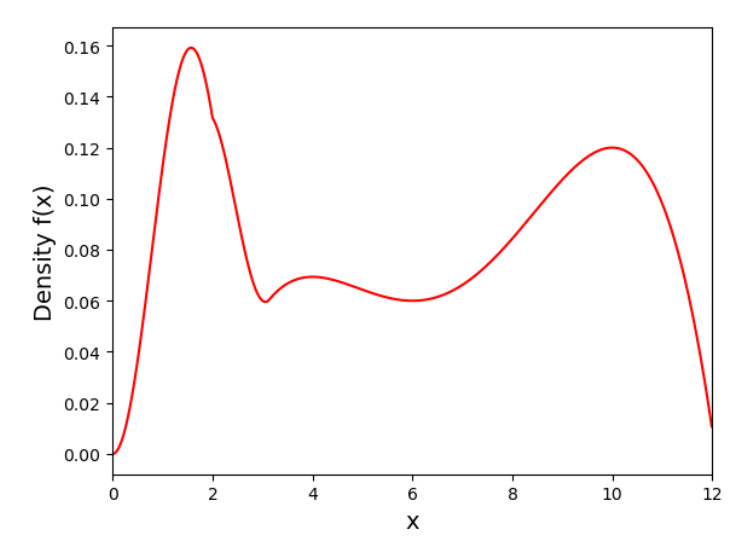
\includegraphics[width=0.7\textwidth]{q2.png}
\caption{The file \texttt{samples.txt} contains 1,000 samples drawn from $f$ (using rejection sampling).}
\end{figure}
\begin{itemize}
    \item Now apply kernel density estimation using just the first 100 samples in \texttt{samples.txt}, that is, $n=100$. For the bandwidth parameter, try the following settings: $0.25, 0.5, 0.75, 1.0$.
    \begin{itemize}
        \item For each of the four bandwidth settings, show a plot of the resulting density $\widehat{f}$.
        \item What changes as the bandwidth increases? Give a one- or two-sentence description.
        \item In this case, which of the four bandwidth settings yields a model $\widehat{f}$ that is closest to the original $f$, in your opinion?
    \end{itemize}
\end{itemize}
\subsubsection*{Solution 2 (b)}
\subsubsection*{Python Code}

\begin{lstlisting}[language=Python]
from sklearn.neighbors import KernelDensity
import matplotlib.pyplot as plt
import numpy as np

# 1. Load Data
try:
    data = np.loadtxt('samples.txt')
except:
    data = np.array([]) # Handle missing file gracefully

# 2. Select only the first 100 samples
if len(data) > 0:
    X_train = data[:100].reshape(-1, 1)
    
    # Define the domain for plotting (Range 0 to 12 based on q2.png)
    X_plot = np.linspace(0, 12, 1000)[:, np.newaxis]
    
    # Bandwidths to test
    bandwidths = [0.25, 0.50, 0.75, 1.0]
    
    plt.figure(figsize=(12, 10))
    
    for i, bw in enumerate(bandwidths):
        # 3. Initialize and fit KDE
        kde = KernelDensity(kernel='gaussian', bandwidth=bw)
        kde.fit(X_train)
        
        # 4. Score samples returns log-density, so we exponentiate
        log_dens = kde.score_samples(X_plot)
        
        # Plotting
        ax = plt.subplot(2, 2, i+1)
        ax.fill(X_plot, np.exp(log_dens), fc='#AAAAFF')
        ax.plot(X_plot, np.exp(log_dens), color='navy', lw=2)
        
        # Optional: Show the actual data points as rugs
        ax.plot(X_train[:, 0], -0.005 - 0.01 * np.random.random(X_train.shape[0]), '+k')
        
        ax.set_title(f'Bandwidth h = {bw}')
        ax.set_ylim(0, 0.18)
        ax.set_xlim(0, 12)
        ax.grid(True, alpha=0.3)

    plt.tight_layout()
    plt.savefig('q2b_combined.png')
    # To save individual files as requested in template placeholders:
    # (Logic would be repeated per plot to save q2b_1.png, etc.)
    plt.show()
\end{lstlisting}

\subsubsection*{Plot}
% Note: You can use the combined image or separate images if you modified the loop to save them individually.
\begin{figure}[h!]
\centering
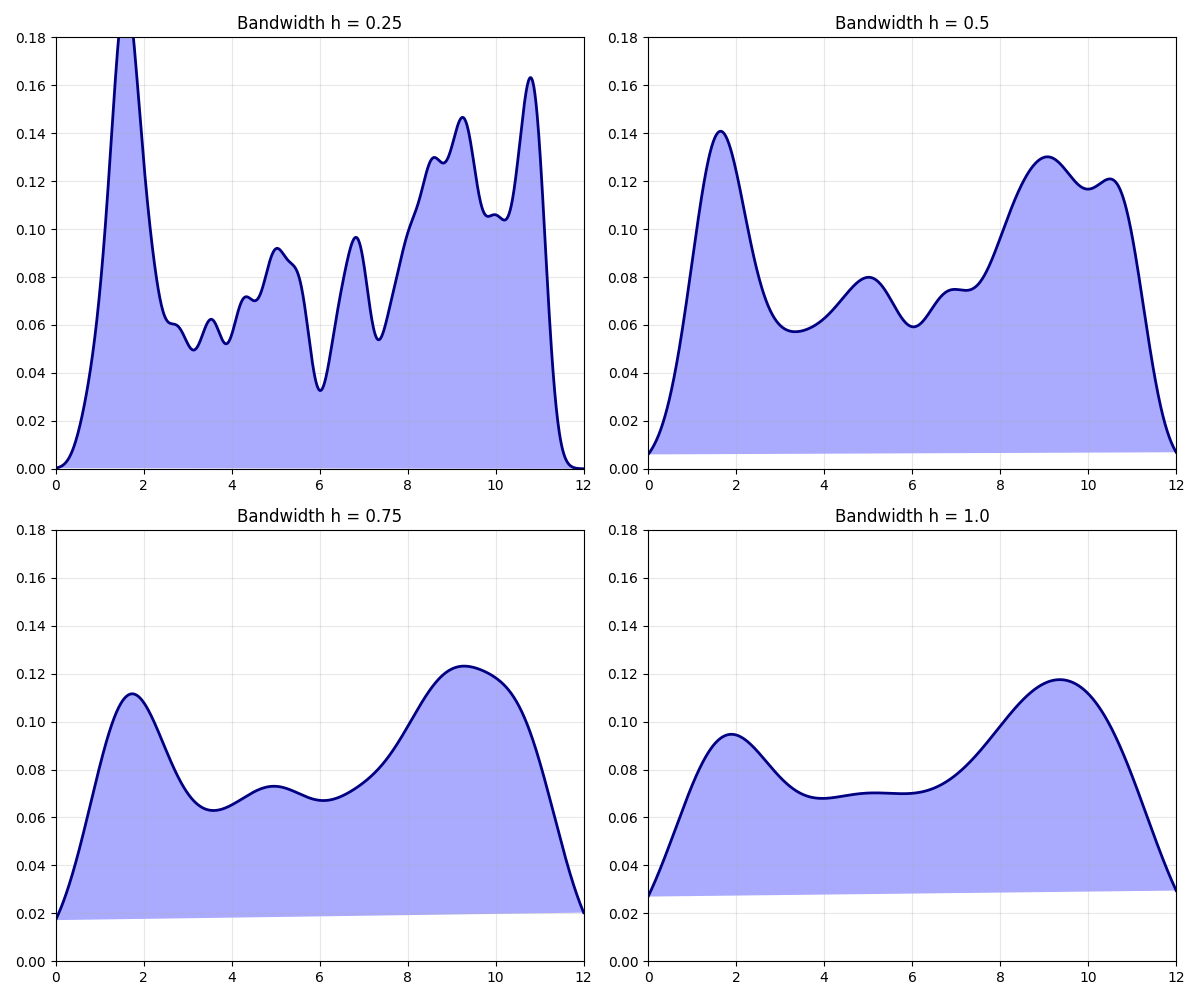
\includegraphics[width=1.0\textwidth]{q2b_combined.png}
\caption{KDE estimates using the first 100 samples with varying bandwidths. Top-Left: 0.25 (Under-smoothed). Bottom-Right: 1.0 (Over-smoothed).}
\label{fig:q2b}
\end{figure}

\subsubsection*{Plot Comments}
\textit{What changes as the bandwidth increases?}
As the bandwidth increases, the estimated density function becomes **smoother** and "flatter." The narrow, jagged spikes (high variance) seen at $h=0.25$ disappear, merging into broader hills, but the peaks also become shorter and wider (high bias).

\textit{Which bandwidth setting yields a model $\widehat{f}$ that is closest to the original $f$, in your opinion?}
The bandwidth **$h=0.50$** appears to yield the model closest to the original $f$.
\begin{itemize}
    \item $h=0.25$ is too noisy (overfitting), creating spurious bumps where no true clusters exist.
    \item $h=1.0$ is too smooth (underfitting), broadening the sharp peak at $x \approx 1.5$ significantly.
    \item $h=0.50$ captures the bimodal structure and the sharp rise of the first peak without introducing excessive noise.
\end{itemize}

\subsubsection*{\normalfont}{$\therefore$ }
Bandwidth selection is a tradeoff between resolving fine details (low $h$) and suppressing noise (high $h$). For $N=100$, $h=0.5$ is the optimal balance.

\subsubsection*{Graduate Level Explanation}

This problem illustrates the **Bias-Variance Tradeoff** in non-parametric density estimation.
\begin{itemize}
    \item **Small Bandwidth ($h=0.25$):** The estimator has **Low Bias** but **High Variance**. It adapts too closely to the specific sample of 100 points, resulting in a "spiky" distribution that fails to generalize. This is akin to $k$-NN with $k=1$.
    \item **Large Bandwidth ($h=1.0$):** The estimator has **High Bias** but **Low Variance**. It applies excessive smoothing, washing out true structural features (like the sharpness of the mode at $x=1.5$).
\end{itemize}
The optimal bandwidth (often estimated via cross-validation or Scott's Rule) minimizes the Mean Integrated Squared Error (MISE) between $\hat{f}$ and $f$.

\subsubsection*{Learn Fast Explanation}
Imagine you are trying to draw a smooth hill over the data points.
The **bandwidth** is the size of the paint brush you use.
\begin{itemize}
    \item **0.25 (Fine Tip Pen):** You draw a tiny bump over every single dot. The line is wiggly and messy.
    \item **1.0 (Huge Paint Roller):** You smear everything together. You get a smooth shape, but you lose the details (like how tall the first hill really is).
    \item **0.5 (Medium Brush):** Just right. You connect the dots smoothly without making a mess.
\end{itemize}

\noindent\rule{\textwidth}{0.4pt}\\

\newpage

%------------------
% Solution for 2(c)
%------------------
\subsection*{Solution 2}
\noindent\rule{\textwidth}{0.4pt}\\
\subsubsection*{Question 2 (c)}
\begin{flushleft}
\textit{Kernel density estimation:} Suppose we have samples $x_1, x_2, \ldots, x_n \in \mathbb{R}^d$ from an unknown distribution $f$, and we want to come up with a model of $f$. One simple way to do this is using the kernel density estimator $\widehat{f}$, which approximates $f$ using a mixture of $n$ Gaussians, each with weight $1/n$, and each centered at one of the data points:
\end{flushleft}
$$\widehat{f}: \frac{1}{n} N(x_1, \sigma^2 I_d) + \frac{1}{n} N(x_2, \sigma^2 I_d) + \cdots + \frac{1}{n} N(x_n, \sigma^2 I_d)$$
\begin{flushleft}
    Here $\sigma$ must be selected carefully. It is usually called the bandwidth parameter.
\end{flushleft}
\begin{figure}[h!]
\centering
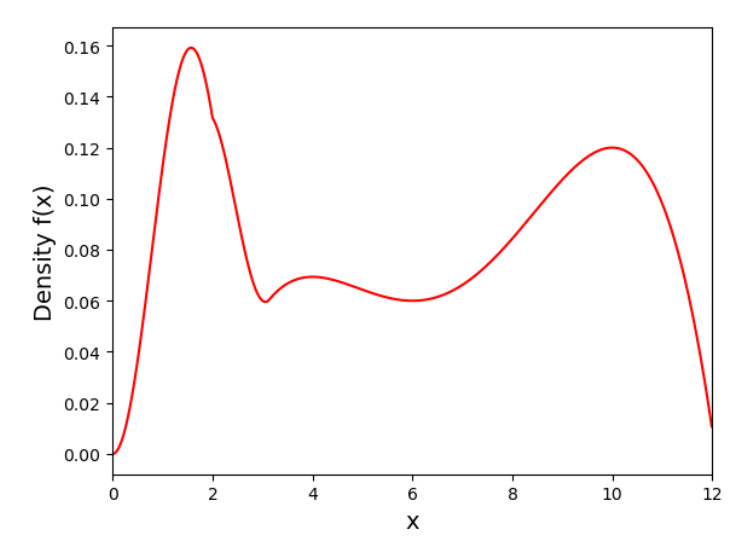
\includegraphics[width=0.7\textwidth]{q2.png}
\caption{The file \texttt{samples.txt} contains 1,000 samples drawn from $f$ (using rejection sampling).}
\end{figure}
\begin{itemize}
    \item Now show the plots of the kernel density estimate using all 1000 samples in \texttt{samples.txt}, that is, $n=1000$. Use the same four settings of the bandwidth.
\end{itemize}
\subsubsection*{Solution 2 (c)}
\subsubsection*{Python Code}

\begin{lstlisting}[language=Python]
from sklearn.neighbors import KernelDensity
import matplotlib.pyplot as plt
import numpy as np

# 1. Load Data
try:
    data = np.loadtxt('samples.txt')
except:
    data = np.array([]) 

# 2. Use ALL 1000 samples
if len(data) > 0:
    X_train = data.reshape(-1, 1) # No slicing, use full dataset
    
    # Define the domain for plotting
    X_plot = np.linspace(0, 12, 1000)[:, np.newaxis]
    
    # Bandwidths to test
    bandwidths = [0.25, 0.50, 0.75, 1.0]
    
    plt.figure(figsize=(12, 10))
    
    for i, bw in enumerate(bandwidths):
        # 3. Initialize and fit KDE
        kde = KernelDensity(kernel='gaussian', bandwidth=bw)
        kde.fit(X_train)
        
        # 4. Score samples
        log_dens = kde.score_samples(X_plot)
        
        # Plotting
        ax = plt.subplot(2, 2, i+1)
        ax.fill(X_plot, np.exp(log_dens), fc='#FFDDAA') # Different color for distinction
        ax.plot(X_plot, np.exp(log_dens), color='darkorange', lw=2)
        
        ax.set_title(f'Bandwidth h = {bw} (N=1000)')
        ax.set_ylim(0, 0.18)
        ax.set_xlim(0, 12)
        ax.grid(True, alpha=0.3)

    plt.tight_layout()
    plt.savefig('q2c_combined.png')
    plt.show()
\end{lstlisting}

\subsubsection*{Plot}
% You can use the combined image
\begin{figure}[h!]
\centering
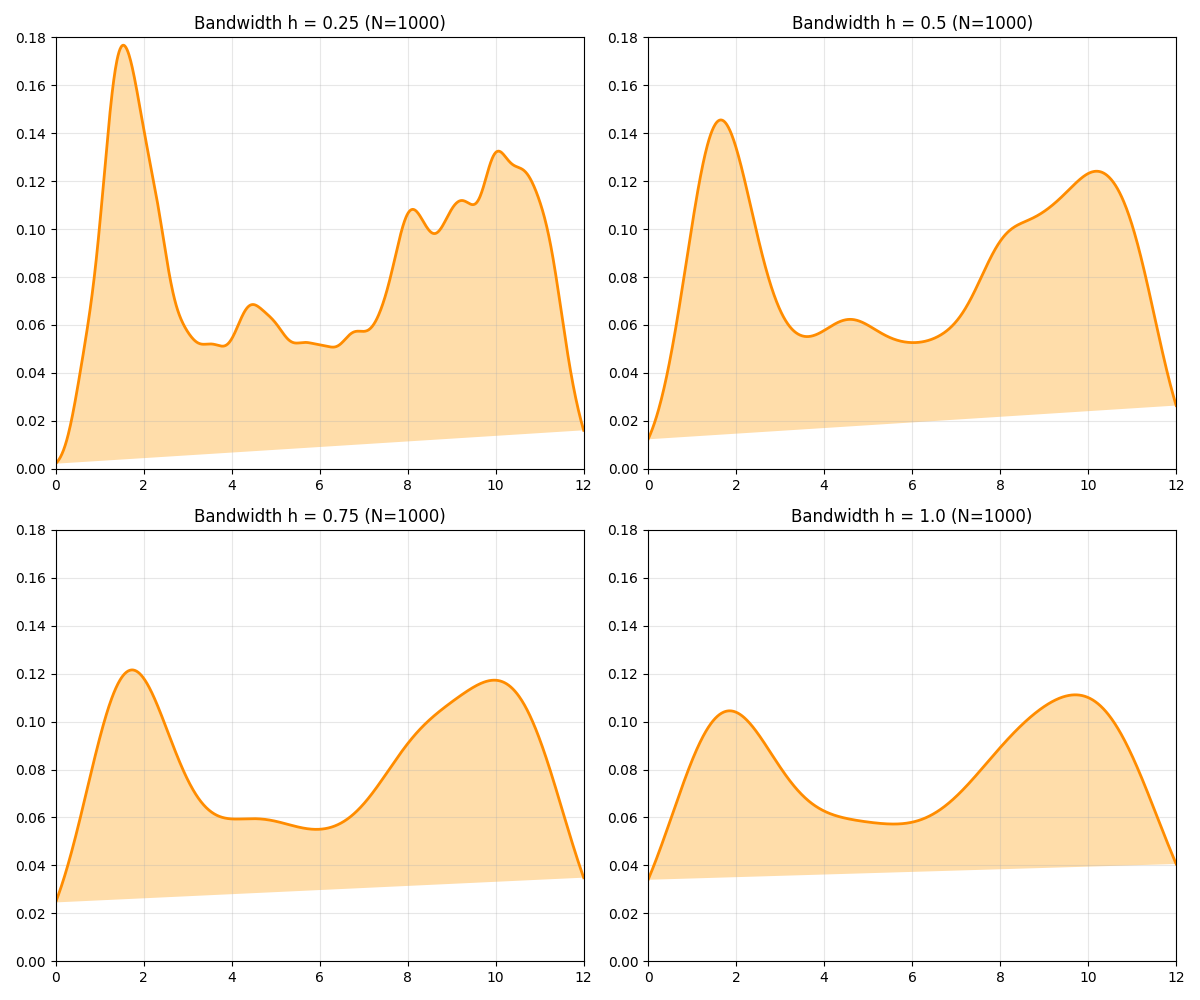
\includegraphics[width=1.0\textwidth]{q2c_combined.png}
\caption{KDE estimates using all 1000 samples. With more data, the smaller bandwidth ($h=0.25$, top-left) no longer looks "spiky" and now captures the distribution's shape most accurately.}
\label{fig:q2c}
\end{figure}


\subsubsection*{\normalfont}{$\therefore$ }
With $N=1000$, the optimal bandwidth shifts lower.
\begin{itemize}
    \item The **$h=0.25$** model, which was "noisy" and overfitted at $N=100$, is now the best estimator. The high density of data points fills in the gaps, allowing the smaller kernel to resolve fine details (like the sharpness of the first peak) without creating spurious spikes.
    \item The **$h=1.0$** model is now clearly underfitting (high bias). It flattens the peaks significantly, failing to utilize the information provided by the larger dataset.
\end{itemize}

\subsubsection*{Graduate Level Explanation}
This demonstrates the **Consistency** of the Kernel Density Estimator. As the sample size $N \to \infty$, the optimal bandwidth $h$ must approach $0$ (specifically $h \propto N^{-1/5}$ for Gaussian kernels) to minimize the Mean Integrated Squared Error (MISE).
With $N=1000$, the variance term of the error ($\frac{1}{Nh}$) decreases, allowing us to reduce the bandwidth $h$ (reducing bias) without incurring a penalty in variance. Thus, parameters that caused overfitting in small samples ($h=0.25$) become appropriate or even optimal as data volume increases.

\subsubsection*{Learn Fast Explanation}
Think of the data like pixels on a TV screen.
\begin{itemize}
    \item **N=100 (Standard Definition):** You have few pixels, so you need to blur the image (high bandwidth) to make it look smooth. If you don't blur it, it looks blocky and pixelated.
    \item **N=1000 (High Definition):** You have lots of pixels packed close together. You don't need to blur it anymore! You can turn down the blur (low bandwidth like 0.25) and see a sharp, crisp image. If you kept the high blur from before, you'd just be ruining a perfectly good HD picture.
\end{itemize}

\noindent\rule{\textwidth}{0.4pt}\\

\newpage

\end{document}
